\chapter{Bayesian Neural Networks}


\section{Bayesian versus frequentist views of learning}\label{sec:bayesian_stat}
In this section we will introduce two concepts of statistical inference. In inferential statistics, the goal is to infer something about a population from data which comes from a sample taken from the population. There are two main approaches in statistical inference, the Bayesian and the Frequentistic paradigm.\\ 
\\
The ideas behind Bayesian statistics goes back to the 18th century and is named after Thomas Bayes (\cite{stigler1986history}). The theory considers probability to reflect uncertainties and belief. Learning is performed by simple applications of rules of probability in particular Bayes' Rule. The results of Bayesian learning are probability distributions over all unknown quantities. On the other hand the conventional frequentistic methodology is to consider the model parameters $\boldsymbol{\theta}$ as fixed but unknown, while the point estimate $\hat{\boldsymbol{\theta}}$ is a random variable, as it is a function of the data set which is assumed to be random and conclusions are made by emphasizing the frequency of the data.
\\
\\
To illustrate the difference between these two methods in more detail, we will consider an example which is often used in the litterateur when comparing these two paradigms, it involves a simple coin toss. There is an uncertainty in this experiment regarding the outcome, will the coin come up heads or tails. This uncertainty can be expressed by the coins probability $p$ of landing on heads, this also often referred to as the bias of the coin. Since the properties of the coin is not known beforehand, we do not know what the exact probability of the coin landing on heads, it could be a fair coin and thus the probability would be $p=\frac{1}{2}$ or it could be an unbalanced coin $p\neq \frac{1}{2}$.\\
\\
A Bayesian statistician would express this uncertainty by a probability distribution over possible values of the unknown probability, and she would then update the distribution as more observations becomes known. On the other hand a frequentist, would find the introduction of a distribution over parameter weights as pure nonsense. The frequentist would instead flip the coin a given number of times to form a data set, and choose some estimator, for the unknown probability $p$ which would be most consistent with the data, an obvious choice would be the relative frequency of heads in the past coin tosses. For example if we flip the coin $n$ times and it has come up heads 70\% of the time, the frequentist would say that this coin is unbalanced whereas the Bayesian would say that it surely looks like the coin is unbalanced, and then update her belief about the coin as more and more flips are repeated. In the next section we will introduce these two paradigms in a more formal way.


\subsection{Maximum Likelihood Estimation}
Let us now consider a data set $\mathbf{X}$, with $n$ examples $x^{(1)}, x^{(2)},\ldots x^{(n)}$ drawn independently form the true but unknown distribution. We let
$L(\mathbf{X};\boldsymbol{\theta})\equiv p(\mathbf{X};\boldsymbol{\theta})$, be parametric family of probability distributions, with parameter $\boldsymbol{\theta}$, which is called the likelihood function. A frequentist is as described earlier trying to find an estimate of the true parameter that have generated the data, we call such an estimate a point estimate and denote $\hat{\boldsymbol{\theta}}$ to separate it from the true parameter. A point estimate can be viewed as a function of data $\hat{\boldsymbol{\theta}}=g(x^{(1)}, x^{(2)},\ldots x^{(n)})$ which is drawn from a random process and thus $\hat{\boldsymbol{\theta}}$ is a random variable.
In most cases of frequentistic inference a point estimate is found by maximizing the likelihood and thus called the maximum likelihood estimate (MLE)
\begin{equation*}
\begin{split}
        \boldsymbol{\boldsymbol{\theta}}_{\text{MLE}}&=\argmax_{\boldsymbol{\theta}}{L(\mathbf{X};\boldsymbol{\theta})}\\
        & = \argmax_{\boldsymbol{\theta}}{\prod^n_{i=1}p(x^{(i)},\boldsymbol{\theta})}
\end{split}
\end{equation*}
It is often more convenient to maximize a sum instead of a product, not only is it easier to handle sums when differentiating but it also helps stabilize the calculations numerically (\cite{Goodfellow-et-al-2016}), thus we take the log of the likelihood function to obtain the log-likelihood function $\ell(\mathbf{X};\boldsymbol{\theta})\equiv \ln{p(\mathbf{X};\boldsymbol{\theta})}$,
\begin{equation*}
\begin{split}
        \boldsymbol{\boldsymbol{\theta}}_{\text{MLE}}&=\argmax_{\boldsymbol{\theta}}{\ell(\mathbf{X};\boldsymbol{\theta})}\\
        &=\argmax_{\boldsymbol{\boldsymbol{\theta}}}{\sum^n_{i=1}\ln{p(x^{(i)},\boldsymbol{\theta})}}
\end{split}
\end{equation*}
and since the logarithm is a monotonic-increasing function, optimizing the log-likelihood is equivalent to optimizing the likelihood. \\
\\
There is two main reasons on why maximum likelihood is considered the preferred estimator to use by frequentist in statistics and machine learning, the MLE is consistent and efficient. We say that an estimator $\hat{\boldsymbol{\theta}}$ is consistent if it converges in probability to the true parameter. That is
\begin{equation*}
    \lim_{n \rightarrow \infty} p\left(\mid\hat{\boldsymbol{\theta}}-\boldsymbol{\theta}\mid > \epsilon\right)=0
\end{equation*}
for all $\epsilon>0$ and an efficient estimator is an estimator that estimates the true parameter of interest in some best possible manner. \\
\\
When data is small, the MLE is often prone to overfitting and regularization methods such as penalized maximum likelihood are applied (see e.g \cite{hastie01statisticallearning}).\\
\\
The sum of squared error in equation \ref{eq:mse} can be justified theoretically by the use of maximum likelihood with a Gaussian likelihood.
To see this consider that we have regression model that output $f(\mathbf{X};\boldsymbol{\theta})=\boldsymbol{\theta}^\top\mathbf{X}$, with real-valued targets $y^{(i)}$ and the likelihood defined as the conditional distribution of $y^{(i)}$ given the data $\mathbf{X}$ and the parameters $\boldsymbol{\theta}$ is gaussian with mean given by the regression output $\hat{y}\equiv f(\mathbf{X};\boldsymbol{\theta})$ and standard deviation $\sigma$, we can thus write
\begin{equation*}
    L(\mathbf{X};\boldsymbol{\theta})=\prod_{i=1}^{N} p\left(y^{(i)} \mid \mathbf{X}^{(i)} ; \boldsymbol{\theta}\right)=\prod_i\frac{1}{\sqrt{2\pi\sigma}}\exp\left(-(\hat{y}^{(i)}-y^{(i)})^2/2\sigma^2\right)
\end{equation*}
Next we take the
logarithm of the likelihood function which gives us the log-likelihood function
\begin{equation*}
\begin{split}
        \ell(\mathbf{X};\boldsymbol{\theta})&=\sum_i\ln\frac{1}{\sqrt{2\pi\sigma}}\exp\left(-(\hat{y}^{(i)}-y^{(i)})^2/2\sigma^2\right)\\
        &=-\frac{n}{2} \ln \sigma^{2}-\frac{n}{2} \ln (2 \pi)-\frac{1}{2 \sigma^{2}} \sum_{i}\left(\hat{y}^{(i)}-y^{(i)}\right)^{2}
\end{split}
\end{equation*}
note that $-\frac{n}{2} \ln \sigma^{2}-\frac{n}{2} \ln (2 \pi)$ does not depend on the model parameters $\boldsymbol{\theta}$ and can thus be omitted when we are maximizing. Maximizing the log-likelihood is the same as minimizing the negative log-likehood, thus we can write 
\begin{equation*}
\begin{split}
        \min_{\boldsymbol{\boldsymbol{\theta}}}{- \ell(\mathbf{X};\boldsymbol{\theta})}=\frac{1}{2 \sigma^{2}} \sum_{i}\left(\hat{y}^{(i)}-y^{(i)}\right)^{2}
\end{split}
\end{equation*}
and since $\frac{1}{2 \sigma^{2}}$ does not depend on $\boldsymbol{\theta}$ either, we can see that minimizing the negative log-likelihood is the same as minimizing the sum of squared error term in equation \ref{eq:mse}.\\
\\
\textcolor{red}{SHOW THAT MAXIMUM LIKELIHOOD IS THE SAME AS CROSS-ENTROPY??}




\subsection{Bayesian learning and prediction}
As we discussed in the introduction to this section: where the frequentist considers the parameter value $\boldsymbol{\theta}$ as fixed but unknown, and the point estimator $\hat{\boldsymbol{\theta}}$ as random variable, the Bayesian perspective on statistics is quite different, since it considers the dataset as being fixed and observable and thus not at all random. On the other hand the true parameter $\boldsymbol{\theta}$ is unknown and thus considered a random variable. \\
In Bayesian modelling, we begin with defining a prior distribution $p(\boldsymbol{\theta})$ over the parameters. This prior distribution expresses our initial view on the parameters, before any data has been observed. When data becomes available, we update our prior distribution to a posterior distribution. The posterior distribution is defined by Bayes' Rule, 
\begin{equation*}
         p(\boldsymbol{\theta}|\mathbf{X},\mathbf{y})=\frac{p(\boldsymbol{\theta})p(\mathbf{X},\mathbf{y}|\boldsymbol{\theta})}{p(\mathbf{X},\mathbf{y})}
\end{equation*}
and it combines the information about the data, that comes from the likelihood function $p(\mathbf{X},\mathbf{y}|\boldsymbol{\theta})$, with the a priori information given by the prior distribution. $p(\mathbf{X},\mathbf{y})$ is called the model evidence and can be interpreted as a normalizing constant given as $p(\mathbf{X},\mathbf{y})=\int p(\mathbf{X},\mathbf{y}\mid \boldsymbol{\theta})p(\boldsymbol{\theta})d\boldsymbol{\theta}$.
We often ignore the normalizing constant and simply writes, 
\begin{equation} \label{eq:posterior}
    p(\boldsymbol{\theta}|\mathbf{X},\mathbf{y})\propto p(\boldsymbol{\theta})p(\mathbf{X},\mathbf{y}|\boldsymbol{\theta})
\end{equation}
An important quality of the Bayesian method, is that is uses a full distribution over the parameters $\boldsymbol{\theta}$ to make predictions. Let us for example consider the case where we have observed a sample consisting of $n$ examples $\mathbf{X}=\boldsymbol{x}^{(1)}, \boldsymbol{x}^{(2)},\ldots, \boldsymbol{x}^{(n)}$, to predict an unobserved label $\boldsymbol{y}^{(n+1)}$ for a new example $\boldsymbol{x}^{(n+1)}$ we need the 
posterior predictive distribution, that is to integrate the model predictions by the posterior
\begin{equation} \label{eq:post_pred_distribution}
    \begin{split}
        &p\left(\boldsymbol{y}^{(n+1)} \mid \boldsymbol{x}^{(n+1)}, \lr{\boldsymbol{x}^{(1)}\boldsymbol{y}^{(1)}}, \ldots, \lr{\boldsymbol{x}^{(n)}, \boldsymbol{y}^{n}}\right)\\
        &=\int p\left(\boldsymbol{y}^{(n+1)} \mid \boldsymbol{\boldsymbol{x}^{(n+1)}, \theta}\right) p \lr{\boldsymbol{\theta} \mid \lr{\boldsymbol{x}^{(1)}, \boldsymbol{y}^{(1)}}, \ldots, \lr{\boldsymbol{x}^{(n)}, \boldsymbol{y}^{(n)}}} \, d \boldsymbol{\theta}
    \end{split}
\end{equation}
This is quite different from the maximum likelihood method, that uses a point estimate for $\boldsymbol{\theta}$ to make predictions on any unobserved data, the Bayesian method takes the uncertainty of estimating $\boldsymbol{\theta}$ into account, which tends to do well in avoidance of overfitting (\cite{Goodfellow-et-al-2016}). The above integral is of an application of the laws of probability (Bayes rule), which makes the Bayesian approach easy to justify theoretically, whereas the frequentist method, is rather based on what \cite{Goodfellow-et-al-2016} calls an ad hoc decision to summarize all knowledge contained in the dataset, with a single point estimator value. \\
An important difference between the Bayesian approach and the MLE, lies on the contribution of a prior distribution. The prior has the effect of shifting the probability mass towards regions of the parameter space, that are preferred a priori. According to \cite{Goodfellow-et-al-2016}, the prior often expresses a preference for models that are simpler or more smooth. Critics of the Bayesian method, often point their finger at the prior distribution, and criticize it for being a subjective component that can affect the predictions of the model. According to \cite{neal2012bayesian} Bayesian methods often do a lot better than a frequentistic model, when training data is limited in availability, but suffers from high computational cost when the number of training examples is large. \\
\\
In many practical examples, the posterior distribution is intractable and therefor must be derived in some other way. Often we will use methods such as Monte Carlo or Variational inference to approximate the posterior distribution. This is of course much more heavy in regard to computational time, then calculating a single point estimate and thus a pendant to MLE is introduced in the next section.



\subsection{Maximum a Posteriori (MAP) Estimation}
One way to come around the computational hurdle it can be to approximate the Bayesian posterior, is to use a point estimate as an approximation. Instead of turning to the frequentist and use the MLE, one can still benefit of the Bayesian method, by allowing the prior to influence the choice of the point estimate. One way of doing this, is to use the maximum a posteriori (MAP) point estimate. The MAP estimate is that value that maximizes the posterior probability,
\begin{equation}\label{eq: MAP}
  \begin{split}
        \boldsymbol{\theta}_{\text{MAP}}&=\argmax_{\boldsymbol{\theta}}{p(\boldsymbol{\theta}\mid x})=\argmax_{\boldsymbol{\theta}}{p(x\mid \boldsymbol{\theta}}) p(\boldsymbol{\theta})\\
        &=\argmax_{\boldsymbol{\theta}}{\ln p(x\mid \boldsymbol{\theta}})+ \ln p(\boldsymbol{\theta})
  \end{split}
\end{equation}
note that the evidence term has been omitted, since it does not depend on the parameter $\boldsymbol{\theta}$ and thus vanishes under maximization anyway. The bottom part of equation \ref{eq: MAP} can be recognized as a equation consisting of the standard log-likelihood term plus a log-prior term. \\
\\
As a nice example consider a model with Gaussian prior placed on the regression weights $\boldsymbol{\theta}$. If we choose specifically the prior to be given by $\mathcal{N}\left(\boldsymbol{\theta},0,\frac{1}{\lambda}\boldsymbol{I}^2\right)$, then the log-prior term in equation \ref{eq: MAP} is proportional to the $L^2$ norm introduced in \ref{eq:L2_reg}, plus a term that does not depend on $\boldsymbol{\theta}$.
Note also that the MAP estimate is the same as the MLE, when choosing a uniform prior, since the $p(\boldsymbol{\theta})$ becomes a constant function in equation \ref{eq: MAP} and consequently we can ignore it when maximizing the expression. MAP estimation has the advantage that it can highlight information through the prior that can not be found through the dataset. According to \cite{Goodfellow-et-al-2016} this additional information, gained from the choice of prior, can reduce the variance in the MAP point estimate in direct comparison with MLE estimate, but this advantage has a price of an increased bias.\\
\\
An obvious disadvantage with MAP estimation, is that we are not going fully Bayesian. A fully Bayesian method is where we marginalize over all possible parameters $\boldsymbol{\theta}$, rather than to optimize and get a single point-estimate. If we want to go full Bayesian, we have to be able to approximate the posterior distribution in some way. \textcolor{red}{Perhaps elaborate, what do we lose by not going "Fully bayesian"?}. \\
\\
MAP is closely related to Bayes optimal estimation that instead of finding the most probable hypothesis (set of parameters) aims to find the most probably label for a new example. The Bayes optimal estimation is done by predicting the $\boldsymbol{y}^{(n+1)}$, which maximizes the predictive posterior in equation \ref{eq:post_pred_distribution}. We do not pursue the idea of Bayes optimal estimation, as we aim to minimize a loss function which is not always equivalent to predicting the most probably label. In this way we preserve the idea that the loss function dictates how much the algorithm should care about making certain predictions as explained in \ref{sec:loss_func}.

\section{Monte Carlo Methods}\label{sec:MC_methods}
When an integral is intractable, we turn to approximations techniques such as Monte Carlo methods. The idea behind Monte Carlo methods is to view the integral as an expectation of some random variable with respect to a probability distribution $p(\cdot)$. Let us consider the case where we have a random variable $\mathbf{x}$ and some function $f(\mathbf{x})$ and we want to approximate the following integral as an expectation under the probability distribution $p(\mathbf{x})$ 
\begin{equation*}
    s=\int p(\mathbf{x}) f(\mathbf{x}) d \mathbf{x}=\mathbb{E}_{p}[f(\mathbf{x})]
\end{equation*}
Now in order to approximate $s$ we can draw samples from the distribution $p(\mathbf{x})$ and approximate the expected value by the empirical average. If we for example draw $n$ samples $\mathbf{x}\sim p(\mathbf{x})$ we can approximate $s$ by $\hat{s}_n$
\begin{equation}\label{eq:empirical_mean_MC}
        \hat{s}_{n}=\frac{1}{n} \sum_{i=1}^{n} f\left(\mathbf{x}^{(i)}\right)
\end{equation}
It is thus possible to a approximate the theoretical expected value, by the empirical mean. This implies the simplest situation, that is, where it is possible to simulate directly from the density, this is often not possible or at least not efficient when facing high-dimensional problems.\\
\\
We can justify this approximation theoretically, by noticing that $\hat{s}_n$ is an unbiased estimator of $s$
\begin{equation*}
    \mathbb{E}\left[\hat{s}_{n}\right]=\frac{1}{n} \sum_{i=1}^{n} \mathbb{E}\left[f\left(\mathbf{x}^{(i)}\right)\right]=\frac{1}{n} \sum_{i=1}^{n} s=s
\end{equation*}
additionally the law of large numbers, states that if the samples $\mathbf{x}^{(i)}$ are independent and identical distributed (i.i.d), the the empirical average converges to the true expectation almost surely
\begin{equation*}
    \lim _{n \rightarrow \infty} \hat{s}_{n}=s
\end{equation*}
this only holds if the variance of the individual terms $\operatorname{Var}[f(\mathbf{x}^{(i)}]$ is bounded. To see this, we note that $\operatorname{Var}[\hat{s}_n]$ converges to 0 if and only if $\operatorname{Var}[f(\mathbf{x}^{(i)}]<\infty$
\begin{equation*}
    \begin{split}
\operatorname{Var}\left[\hat{s}_{n}\right] &=\operatorname{Var}\left[\frac{1}{n} \sum_{i=1}^{n} f(\mathbf{x}^{(i)})]\right] \\ &=\frac{1}{n^{2}} \sum_{i=1}^{n} \operatorname{Var}[f(\mathbf{x}^{(i)})]
=\frac{\operatorname{Var}[f(\mathbf{x})]}{n}
\end{split}
\end{equation*}
Further the central limit theorem states that, if $\mathbb{E}[f(\mathbf{x})]=s$ and $\operatorname{Var}[f(\mathbf{x})]<\infty$ then
\begin{equation*}
    \frac{\hat{s}_{n}-s}{\sqrt{\operatorname{Var}[f(\mathbf{x})] / n}} \stackrel{D}{\rightarrow} \mathcal{N}(0,1)
\end{equation*}
which is equivalent to
\begin{equation*}
    \hat{s}_n\sim \mathcal{N}\left(s,\frac{\operatorname{Var}[f(\mathbf{x})]}{n}\right)
\end{equation*}
When it is not possible to make simulations of $\mathbf{x}$ directly, either because the distribution $p(\mathbf{x})$ is intractable or because sampling from $p(\mathbf{x})$ is computationally infeasible, Markov Chain Monte Carlo methods are used, which in short is based on simulating from a target distribution by running a Markov Chain that eventually will converge and have the target distribution as its stationary distribution. Markov Chain Monte Carlo methods will be examined more thoroughly in section \ref{sec:MCMC}.

\section{A Simple Bayesian Neural Network} \label{sec:simple_BNN}

\begin{figure}
    \centering
    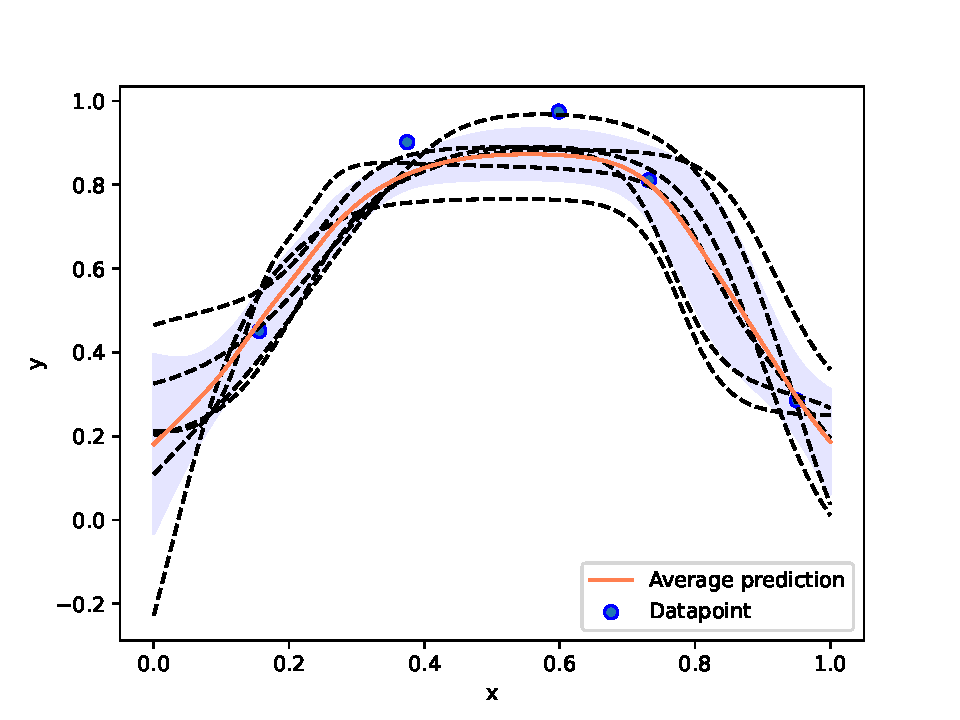
\includegraphics[width=\textwidth,height=\textheight,keepaspectratio]{pics/figure_simple_BNN.pdf}
    \caption{Sampled neural networks from a predictive posterior that is based on a Gaussian prior and a Gaussian likelihood on the 6 datapoints. The average prediction of the networks are plotted along with a filled area defined by the average plus minus the standard deviation of the network predictions to represent uncertainty.}
    \label{fig:simple_BNN}
\end{figure}

\noindent
A simple example, inspired by \cite{neal2012bayesian}, will illustrate the general concept of Bayesian learning for neural networks and the inefficiency of brute force methods. Figure \ref{fig:simple_BNN} shows 6 BNNs whose weights and biases were drawn from independent standard normal prior distributions except output weights, which had a standard deviation of $\frac{1}{\sqrt{16}}$. The networks performs regression on 6 datapoints for which the prior and the likelihood was based. \\
\\
The 6 networks was chosen from a larger pool of $10^5$ networks whose weights and biases were sampled from identical prior distributions. The likelihood was computed for each of these networks and scaled so that the largest likelihood was 1. The networks were then accepted with the probability of this scaled likelihood for which only 6 was accepted. This approach resembles rejection sampling and embodies the posterior in \ref{eq:posterior} by making the prior control the generation of candidate networks and the likelihood control which of these candidates are rejected.\\
\\
We follow the suggestion of \cite{neal2012bayesian} to model regression tasks with a conditional distribution for the real valued targets $\boldsymbol{y}_k$, from $k$ neural networks with outputs $f_k(\boldsymbol{x})$, defined by a Gaussian 
\begin{equation}\label{eq:regr_taget_distribution}
    p(\boldsymbol{y} \mid \boldsymbol{x}) = \prod_k \frac{1}{\sqrt{2 \pi} \sigma_k} \exp{- \frac{\lr{f_k(\boldsymbol{x}) - y_k}^2}{2 \sigma_k^2}}
\end{equation}
with mean $f_k(x)$ and standard deviation $\sigma_k$ as a hyperparameter, which we chose to be $\sigma_k = 0.1$ for all $k$.
\\
\\
The optimal way to predict the target associated with various new examples, assuming we want to minimize the expected squared error, is to predict the mean of the predictive distribution in equation \ref{eq:post_pred_distribution}. For a regression model defined by equation \ref{eq:regr_taget_distribution} this is equal to predicting 
\begin{equation*}
    \hat{\boldsymbol{y}}^{(n+1)} = \int f\lr{\boldsymbol{x}^{(n+1)}, \boldsymbol{\theta}} p\lr{\boldsymbol{\theta} \mid \lr{\boldsymbol{x}^{(1)}, \boldsymbol{y}^{(1)}}, \dots, \lr{\boldsymbol{x}^{(n+1)}, \boldsymbol{y}^{(n+1)}}} \, d \boldsymbol{\theta}
\end{equation*}
As we can only sample from this distribution we resort to a Monte Carlo approximation by averaging over the 6 functions drawn from the posterior as in equation \ref{eq:empirical_mean_MC}. This is also equivalent to minimizing mean squared error. The average is shown in \ref{fig:simple_BNN} by the dotted line. But Bayesian inference can do more than a single-valued guess. By examining the function we can also see the uncertainty of the guesses, for example how rapidly uncertainty increases beyond the region of the datapoints. 
\\
\\
\textcolor{red}{Add text on how we don't need to regularize, and make a train/test split and other perks of BNNs that Neal mentions (perhaps just refer to him instead of showing/arguing for them. MacKay1991 mentions that BNN applies Occams Razor automatically.}\\
\\
This shows some of the perks of using Bayesian inference for neural networks, but what remains is the downside of computational time. Generating $10^5$ samples to get 6 draws from the posterior not very efficient and this only becomes more infeasible as the number of datapoints increase. In section \ref{sec:MCMC} we discuss how to sample more effectively from the posterior using Markov-Chain Monte Carlo methods and in \ref{sec:ADVI} we introduce the approach of variations inference for approximating intractable integrals. Another unresolved matter is how to choose the prior, and how this choice affects our results. This is discussed in \ref{sec:priors} while how to efficiently choose the parameters of the prior is discussed in \ref{sec:hier_models}.


\section{Priors}\label{sec:priors}
From section \ref{sec:bayesian_stat} and the example given in section \ref{sec:simple_BNN} it is seen that Bayesian inference starts with a prior for the model parameters, which is suppose to embody ones prior beliefs about the assigned task. However in neural networks the relationship between parameters and the problem can be very abstract and not as intuitive as in other machine learning models like linear regression models or SVMs. \\
\\
\cite{neal2012bayesian} stresses that even though it can seem like BNNs can be threatened by a lack of a suitable prior this is not the case, as much past work shows useful criteria for selecting suitable priors, even without full understanding of what the prior over the parameters will mean in terms of the output of the network. \cite{mackay1991} and \cite{MacKay1992} has produced results, that Neal describes as at least reasonable, by giving the parameters Gaussian prior distributions. He lets the variance of these distribution be selected as a hyperparameter, which allows the model to adapt to the data. We must state however, that we do not suggest that this is the correct prior to use, as each learning problem is unique. In his work MacKay emhasizes the advantage of hierachichal models described in section \ref{sec:hier_models}.\\
\\
In a BNN the role of the hyperparameters for the priors of the parameters correspond roughly to he role of the weight decay constant $\alpha$ in equation \ref{eq:reg_obj_func} used in training of a conventional neural network. But as noted by \cite{neal2012bayesian} these hyperparameters in BNNs can be found without the need for a validation set.



\section{Hierarchical Models} \label{sec:hier_models}
\textcolor{red}{TÆNKER VI KAN SKRIVE LIDT OM HIERAKISKE MODELLER OGSÅ - KAN EVENTUELT FLYTTES ANDET STEDS HEN HVIS DET PASSER BEDRE.}

\clearpage
\section{Markov chain Monte Carlo}\label{sec:MCMC}
 As we mentioned in section \ref{sec:bayesian_stat} the posterior distribution is often intractable and therefore not possible to derive any analytical solution of it. Therefor we need simulation based methods. We want to be able to calculate posterior summaries like $\mathbb{E}_p\left[f(\boldsymbol{\theta})\right]$ where $f(\boldsymbol{\theta})$ is our model and the expectation is taking under the posterior distribution. Such an expectation is straight forward to approximate when dealing with nice and low dimensional distributions, with simple Monte Carlo methods as described in section \ref{sec:MC_methods}. Other Methods like importance sampling has often been proposed in the litterateur for simple problems, but rarely for high-dimensional problems as we face with Neural Networks.
 \\
 \\
 For more complex models, these methods are not at all useful in practise, a more relevant collection of methods, are the
 Markov chain Monte Carlo (MCMC) methods. The main idea is to simulate a Markov chain, which has the posterior distribution as it's stationary distribution. As a discussion of the different MCMC methods would be rather hard to understand without the fundamental knowledge of Markov chains, we will summarize the most important concepts in the next section. The curious reader is encouraged to see \cite{lawler2006introduction} for a deeper discussion of this subject.
 
\subsection{Definition and Basic Results for Markov chains}
First we define a stochastic process, which is a set of random variables that are defined over some probability space $\left\{X^{(t)} \right\}_{t\in T}$, where $T\subset \mathbb{R}$ is the indexation and may be considered as a temporal or a time index. In the context of Machine Learning, the set $T$ can be interpreted as the iterations of a simulation scheme. In stochastic simulation we typically have that $T=\mathbb{N}$ and we can write the stochastic process as $\left\{X^{(n)}\right\}_{n\geq 0}$, where $n$ reminds us that we have discrete index set. Throughout this thesis we will only consider discrete time stochastic processes, since this is most relevant when discussing stochastic simulation. \\
The set $\mathbb{S}$ is the space of the process $\left\{X^{(n)} \right\}_{n\geq 0}$, and denoted the state space. The state space can be any mathematical set, but in most applications it is the set of integers $\mathbb{N}$ or numbers on the real line $\mathbb{R}$.\\
\\
In Bayesian modelling we consider the model parameters $\boldsymbol{\theta}$ as a random variable and therefor, we can consider a sequence of generated model parameters as a stochastic process. In this section we introduce the basic theory, and we will let $\{\boldsymbol{\theta}^{(n)}\}_{n\geq 0}$ denote the stochastic process of interest.\\ \\
The objective with the BNN model is as early mentioned to make predictions for some unknown test cases. For this we either need the posterior predictive distribution from equation \ref{eq:post_pred_distribution} which is often not possible to derive analytically or we might be interested in an expectation of a model with respect to the posterior distribution.
We call the distribution we wish to sample from the target distribution and denote it $\hat{p}(\cdot)$. The target distribution in Bayesian statistics in often the posterior and thus $\hat{p}(\boldsymbol{\theta})\equiv p(\boldsymbol{\theta}\mid \mathbf{X},\mathbf{y})$. Let us now assume we want to calculate an expectation of some function $\alpha(\boldsymbol{\theta})\equiv f_i(\mathbf{x}^{(n+1)};\boldsymbol{\theta})$ with respect to the target distribution, that is
\begin{equation}\label{eq: expectation_under_posterior}
    \mathbb{E}\left[\alpha(\boldsymbol{\theta})\right]=\int \alpha(\boldsymbol{\theta})\hat{p}(\boldsymbol{\theta}) d\boldsymbol{\theta}
\end{equation}
In section \ref{sec:MC_methods} we saw that such an expectation can be approximated by the empirical average, where we have drawn $\boldsymbol{\theta}$ from the target distribution $\hat{p}(\boldsymbol{\theta})$. The draws in simple Monte carlo methods are i.i.d, which is a very inefficient way of drawing samples when the target distribution is complex, often this is not even a possibility.\\
\\
Another way is generate a sequence of dependent variables $\boldsymbol{\theta}^{(n)}$, such a sequence is often generated by simulating a stochastic process $\{\boldsymbol{\theta}^{(n)}\}_{n\geq 0}$ and not an arbitrary stochastic process, but a process that satisfies the Markov property. The Markov property states that to make predictions about a future state of the system, it suffices to consider only the present state of the system and not all the past states. Such a process is called a Markov chain, named after the famous mathematician Andrey Markov. Formally we can write this as $ \boldsymbol{\theta}^{n} \independent (\boldsymbol{\theta}^0,\boldsymbol{\theta}^1, \ldots, \boldsymbol{\theta}^{n-2}) \mid \boldsymbol{\theta}^{n-1}$. The Markov chain is defined by an initial distribution for the first state of the chain $\boldsymbol{\theta}^{(0)}$, and transition probability/density for the next states in the system. We write the transition probability from transitioning from state $\boldsymbol{\theta}$ to another state $\boldsymbol{\theta}^\prime$ as $T(\boldsymbol{\theta}^\prime\mid \boldsymbol{\theta})$. \\
\\
When drawing samples from the stochastic process $\{\boldsymbol{\theta}^{(n)}\}_{n\geq 0}$ we want to make sure that draws are actually coming from the desired distribution $\hat{p}(\boldsymbol{\theta})$ no matter the initial probability. To do this we need the fact that if a Markov chain has a stationary distribution $\pi(\boldsymbol{\theta})$, and reach a state of the chain where this distribution is established the distribution persists. That is if $\boldsymbol{\theta}^{(n)}$ has $\hat{p}(\boldsymbol{\theta})$ as it's distribution, then  $\boldsymbol{\theta}^{(n^\prime)}$ will have the same distribution, and this will hold for all $n^\prime\geq n$. Formally we call this property, the invariance property,
\begin{equation*}
    \pi(\boldsymbol{\theta}^\prime)=\int T(\boldsymbol{\theta}^\prime\mid \boldsymbol{\theta}) \pi(\boldsymbol{\theta})d\boldsymbol{\theta}
\end{equation*}
A sufficient, but not necessary condition that ensures that a particular $\hat{p}(\boldsymbol{\theta})$ is the desired stationary distribution is the detailed balance condition. The condition states if we let $T(\cdot,\cdot)$ be a transition probability which satisfies the following condition $\hat{p}(\boldsymbol{\theta})T(\boldsymbol{\theta}, \boldsymbol{\theta}^\prime) = \hat{p}(\boldsymbol{\theta}^\prime)T(\boldsymbol{\theta}^\prime, \boldsymbol{\theta})$, then $\hat{p}(\cdot)$ is a stationary distribution of the Markov chain associated with the transition probability $T(\cdot,\cdot)$. The detailed balanced condition is proved below, 
\begin{proof}
Suppose that a distribution $\hat{p}(\cdot)$ satisfies the condition of the detailed balance theorem. Then
 \begin{equation*}
     \begin{split}
         &\hat{p}(\boldsymbol{\theta})T(\boldsymbol{\theta},\boldsymbol{\theta}^\prime)= \hat{p}(\boldsymbol{\theta}^\prime)T(\boldsymbol{\theta}^\prime,\boldsymbol{\theta}) \Leftrightarrow \\
          &\int\hat{p}(\boldsymbol{\theta})T(\boldsymbol{\theta},\boldsymbol{\theta}^\prime)d\boldsymbol{\theta}=\int \hat{p}(\boldsymbol{\theta}^\prime)T(\boldsymbol{\theta}^\prime,\boldsymbol{\theta}) d\boldsymbol{\theta} \\
         &= \hat{p}(\boldsymbol{\theta}^\prime)\int T(\boldsymbol{\theta}^\prime,\boldsymbol{\theta})d\boldsymbol{\theta} =\hat{p}(\boldsymbol{\theta}^\prime)
     \end{split}
\end{equation*}
where we have used that $\int T(\boldsymbol{\theta}^\prime,\boldsymbol{\theta})d\boldsymbol{\theta}=1$ since the probability of transitioning from state $\boldsymbol{\theta}^\prime$ to any possible state $\boldsymbol{\theta}\in\mathbb{S}$ must be equal to one. 
\end{proof}
A Markov chain there is ergodic has a unique stationary distribution from which it converges to from any initial state (see e.g \cite{turkman2019computational}). For a Markov chain to be ergodic, we need two conditions for the states of the system and the transition probabilities. These conditions are known as irreducibility and aperiodicity. If we can create an ergodic Markov chain, with transition probabilites satifying the detailed balance condition, we can approximate expectations like the one in equation \ref{eq: expectation_under_posterior} with an empirical average like in equation \ref{eq:empirical_mean_MC},
\begin{equation*}
    \mathbb{E}\left[a(\boldsymbol{\theta})\right]\approx \frac{1}{n}\sum_{i=0}^n a(\boldsymbol{\theta}^{(i)})
\end{equation*}
where $\boldsymbol{\theta}^{(0)},\ldots \boldsymbol{\theta}^{(n)}$ being the states of the chain. Often we discard or burn some of the initial states, since these may not be representative of the desired distribution since the chain has not reached the stationary distribution yet, such a procedure is called burning in the Markov chain. When the chain has reached the stationary distriubtion, it is possible to draw as many identical distributed samples as we wish for, but one should note that any successive samples will be highly correlated with each other and thus not necessarily a good representative for the target distribution. \cite{Goodfellow-et-al-2016} suggest a way to come around this problem, by only returning every n successive sample. Because of both the burning in phase and the time required for the chain to return uncorrelated samples, MCMC is often computational expensive. \\
\\
In order to produce truly independent samples, \cite{Goodfellow-et-al-2016} suggest to run multiple Markov chains in parallel and explains that practitioners often uses a number of chains that are run in parallel, similar to the number of examples in a minibatch and then draw the samples needed from this set of Markov chains. \\
\\
In the next section we will cover a very useful way of generating a Markov chain that converges to the target distribution. 


\subsection{The Metropolis algorithm} \label{sec:Metropolis_Hastings}
The Metropolis algorithm is a Markov chain Monte Carlo (MCMC) method, which is used to sample from a Bayesian posterior. 
The Metropolis (MH) algorithm was originally introduced by \cite{Metropolis1953} and was developed to simulate the states for a system of idealized molecules (\cite{neal2012mcmc}). This was later further developed by \cite{hastings70}, so that the algorithm could now simulate from a general distribution and not just a symmetric one, as it was previously based on. Due to its versatility and simplicity, the Metropolis algorithm is one of the most widely used in MCMC methods.\\
\\
The Metropolis algorithm generates a sequence of stochastic variables by sampling from a probability distribution, more specific the samples are drawn from a proposal distribution, that specifies the probability of moving to a new point in the sample space. \\
As mentioned in section \ref{sec:MCMC}, the main idea is to create a Markov chain that will converge towards a given distribution, so that the target distribution becomes the Markov chain's stationary distribution.  \\
\\
The simple Metropolis algorithm introduced in the original paper by \cite{Metropolis1953} consider a target distribution $\hat{p}(\boldsymbol{\theta})$ and a proposal distribution $q(\boldsymbol{\theta})$. The algorithm generates a Markov chain, by starting the chain at some arbitrarily point generated from the proposal distribution $\boldsymbol{\theta}^{0}\sim q(\boldsymbol{\theta})$ and then proposing a candidate state for the next state in the chain $\boldsymbol{\theta}^{(cand)}$, where this candidate state is drawn from the conditional distribution on the previous state $\boldsymbol{\theta}^{(cand)}\sim q(\boldsymbol{\theta}^{(n+1)}\mid\boldsymbol{\theta}^{(n)})$, and then we decide whether or not to reject this new state based on the relative probability density to the old state. If the relative density is larger than one, we accept the new state, if the relative density is less than one, we accept the new state with probability $\frac{p(\boldsymbol{\theta}^{cand})}{p(\boldsymbol{\theta}^{(n)})}$. The algorithm is written in pseudo code in algorithm \ref{algo_2}.
% Metropolis Algorithm
\begin{algorithm}[h!]\label{algo_2}

\SetAlgoLined
initialize $\boldsymbol{\theta}^0\sim q(\boldsymbol{\theta})$;

\For{$i=1,2,\ldots$}{
Propose: $\boldsymbol{\theta}^{c a n d} \sim q\left(\boldsymbol{\theta}^{(i)} \mid \boldsymbol{\theta}^{(i-1)}\right)$

Acceptance Probability:

$ \alpha\left(\boldsymbol{\theta}^{c a n d} \mid \boldsymbol{\theta}^{(i-1)}\right)=\min \left\{1, \frac{p\left(\boldsymbol{\theta}^{c a n d}\right)}{ p\left(\boldsymbol{\theta}^{(i-1)}\right)}\right\} $

$u \sim  \text { Uniform }(0,1)
$

  \uIf{$u<\alpha$}{
    Accept the proposal: $\boldsymbol{\theta}^{(i)} \leftarrow \boldsymbol{\theta}^{c a n d}$\;
  }
  \Else{
    Reject the proposal: $\boldsymbol{\theta}^{(i)} \leftarrow \boldsymbol{\theta}^{(i-1)}$ \;
  }
    }
\caption{Metropolis algorithm}
\end{algorithm}\\
In the original algorithm the proposal distribution must satisfy the symmetry condition,
\begin{equation*}
    q(\boldsymbol{\theta'}\mid \boldsymbol{\theta})=q(\boldsymbol{\theta}\mid \boldsymbol{\theta'})
\end{equation*}
To show that this works out, and we are in fact sampling from the target distribution, we must show that these transitions from one state to another in the Markov chain leaves the target distribution invariant. For $\boldsymbol{\theta'}\neq \boldsymbol{\theta}$ the algorithm leads to the following transitions densities,
\begin{equation*}
    T\left(\boldsymbol{\theta}' \mid \boldsymbol{\theta}\right)=q\left(\boldsymbol{\theta}' \mid \boldsymbol{\theta}\right) \min \left(1, p\left(\boldsymbol{\theta}'\right) / \hat{p}(\boldsymbol{\theta})\right)
\end{equation*}
The detailed balance condition is thus verified by,
\begin{equation*}
\begin{aligned}
T\left(\boldsymbol{\theta}' \mid \boldsymbol{\theta}\right) \hat{p}(\boldsymbol{\theta}) &=q\left(\boldsymbol{\theta}' \mid \boldsymbol{\theta}\right) \min \left(1, p\left(\boldsymbol{\theta}'\right) / \hat{p}(\boldsymbol{\theta})\right) \hat{p}(\boldsymbol{\theta}) \\
&=q\left(\boldsymbol{\theta}' \mid \boldsymbol{\theta}\right) \min \left(\hat{p}(\boldsymbol{\theta}), \hat{p}\left(\boldsymbol{\theta}'\right)\right) \\
&=q\left(\boldsymbol{\theta} \mid \boldsymbol{\theta}'\right) \min \left(\hat{p}\left(\boldsymbol{\theta}'\right), \hat{p}(\boldsymbol{\theta})\right) \\
&=q\left(\boldsymbol{\theta} \mid \boldsymbol{\theta}'\right) \min \left(1, \hat{p}(\boldsymbol{\theta}) / \hat{p}\left(\boldsymbol{\theta}'\right)\right) \hat{p}\left(\boldsymbol{\theta}'\right) \\
&=T\left(\boldsymbol{\theta} \mid \boldsymbol{\theta}'\right) \hat{p}\left(\boldsymbol{\theta}'\right)
\end{aligned}
\end{equation*}
the transitions proposed by the algorithm thus leaves the target distribution $\hat{p}(\boldsymbol{\theta})$ invariant and thus samples produced by this Markov chain all has the same stationary distribution $\hat{p}(\boldsymbol{\theta})$. One problem arises since the algorithm needs to calculate the relative density of $\frac{p(\boldsymbol{\theta'})}{p\left(\boldsymbol{\theta}\right)}$, but our target distribution is often intractable and thus a analytical solution is not possible. But since the algorithm only need the target distribution for calculating the relative density, we can use that we know that the posterior is equal to the likelihood times the prior up to some constant of normalization and thus we can use this instead of the target distribution directly.\\
\\
The Metropolis algorithm has been used in many application within Bayesian Statistics and often with good results. One major disadvantage with the algorithm is that it produces highly correlated samples as we discussed about MCMC methods in general in section \ref{sec:MCMC}. One way to cope with this problem is to throw away some of the samples or run multiple chains in parallel.\\
\\
A very common feature of the algorithm is the random-walk behavior (\cite{gelmanbda04}). The simulations generated by the Markov chain is often zigging and zagging through the target distribution in a very inefficient way. This can be seen very clearly in figure \ref{fig:MH_sampling}, where 500 samples from the Metropolis algorithm has been generated for a bivariate target distribution with mean $\boldsymbol{\mu}=\left[\begin{array}{l}
0, 
0
\end{array}\right]^\top$ and covariance matrix
$\boldsymbol{\Sigma}=\left[\begin{array}{cc}
1 & 0.6\\
0.6 & 1
\end{array}\right]$\footnote{The python code can be found in appendix \ref{app:MH_code}}. \\
\\
A more generalized version of the algorithm is the one introduced by \cite{hastings70}, which allows for non-symmetric proposal distributions, that is $q(\boldsymbol{\theta}^\prime\mid \boldsymbol{\theta}) \neq q(\boldsymbol{\theta}\mid \boldsymbol{\theta}^\prime)$. To correct for this asymmetry in the proposal distribution, the acceptance ratio is replaced by
\begin{equation}\label{eq: hasti_pasti}
\alpha\left(\boldsymbol{\theta}^{c a n d} \mid \boldsymbol{\theta}^{(i-1)}\right)=\min \left\{1, \frac{q\left(\boldsymbol{\theta}^{(i-1)} \mid \boldsymbol{\theta}^{c a n d}\right) \hat{p}\left(\boldsymbol{\theta}^{c a n d}\right)}{q\left(\boldsymbol{\theta}^{c a n d} \mid \boldsymbol{\theta}^{(i-1)}\right) \hat{p}\left(\boldsymbol{\theta}^{(i-1)}\right)}\right\} 
\end{equation}
One should note that the Metropolis algorithm is an instance of the generalized version, since equation \ref{eq: hasti_pasti} is identical to the acceptance ratio in the original algorithm when allowance for a symmetric distribution. \\
\\
The introduction of an asymmetric proposal distribution, is often useful when we want to increase the speed of the random walk generated by Metropolis algorithm, but this is often not sufficient for complicated models with high-dimensional target distributions as we face with Bayesian Neural Networks (\cite{gelmanbda04}). We will in the next chapter concentrate on a more efficient way of simulating the chain.
\begin{figure}
    \centering
    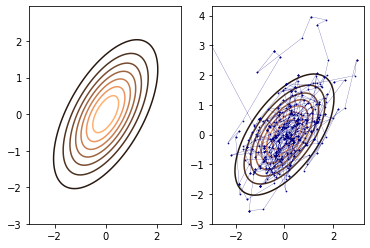
\includegraphics{pics/mh_randomWalk_behavior.png}
    \caption{500 samples generated with the Metropolis Hasting algorithm. The target distribution is a bivariate normal distribution. \textcolor{red}{Make similar y-axis}}
    \label{fig:MH_sampling}
\end{figure}
\clearpage
\section{Hamiltonian Monte Carlo}
As we mention in section \ref{sec:Metropolis_Hastings}, a significant inefficiency in the Metropolis algorithm, is that it often behaves like a random walk and thus the simulations take a longer road while moving through the target distribution, which gives rise to slow simulation. This is espacially a problem when concerning high-dimensional problems, such as Bayesian Neural Networks (\cite{neal2012bayesian}).
Another way to generate proposals with a higher efficiency, is in which the network weights are updated dynamically by simulating Hamiltonian dynamics and then use the Metropolis algorithm to accept or reject these proposals.This algorithm suppress the local random walk behavior and thus allowing it to move much faster and more rapidly through the distribution. The method presented is called Hamilton Monte Carlo (HMC), and is commonly used in computational physics and statistics. The algorithm was originally proposed by \cite{Duane1987216} for calculations used in lattice quantum chromodynamics, but was later introduced to the world of statistics when it was used for Bayesian Neural Networks n \cite{neal2012bayesian}\\
\\
The HMC algorithm reduces correlation between successive sampled states, compared to the Metropolis Hastings algorithm in section \ref{sec:Metropolis_Hastings}, by proposing moves to distant states which maintain a high probability of acceptance due to the approximate energy conserving properties of the simulated Hamiltonian dynamic when using a symplectic integrator\footnote{In mathematics, a symplectic integrator is a numerical integration scheme for Hamiltonian systems.}. The reduced correlation means fewer Markov chain samples are needed to approximate integrals with respect to the target probability distribution for a given Monte Carlo error. For the HMC algorithm we need to construct a differential equation system, that is known to keep the target distribution invariant. If we can achieve this, we can simulate transitions following the solution to this differential equation system and these transitions can be shown to leave the target distribution invariant. Such a differential equations system is often the Hamiltonian dynamics named after William Rowan Hamilton and will be introduced in the next section. 

\subsection{Hamiltonian dynamics}
Before we move to the actual HMC algorithm, we need to become familiar with the concept of Hamiltonian dynamics. Hamiltonian dynamics are used to describe how an object move around in a system. The Hamiltonian dynamics is define by the objects location $\boldsymbol{\theta}\in \mathbb{R}^d$ and it's momentum $\boldsymbol{\rho}\in \mathbb{R}^d$, which in the physics are equivalent to an object's mass times it's velocity at some point in time $t$. The object's location is associated with a potential energy $U(\boldsymbol{\theta})$ and likewise the momentum is associated with a kinetic energy $K(\boldsymbol{\rho})$. The sum of the potential and kinetic energy is regarded as the total energy of the system and often called the Hamiltonian,
\begin{equation*}
H(\boldsymbol{\theta},\boldsymbol{\rho})=U(\boldsymbol{\theta})+K(\boldsymbol{\rho})    
\end{equation*}       
one important feature of the Hamiltonian is that it is constant over time. Taking the partial derivative with respect to time of the location and momentum, shows us how they evolve over time,
\begin{equation}\label{eq:hamilton_equations}
\begin{split}
\frac{d \theta_{i}}{d t}=\frac{\partial H}{\partial \rho_{i}}=\frac{\partial K(,\boldsymbol{\rho})}{\partial \rho_{i}} \\
\frac{d \rho_{i}}{d t}=-\frac{\partial H}{\partial \theta_{i}}=-\frac{\partial U(,\boldsymbol{\theta})}{\partial \theta_{i}}
\end{split}
\end{equation}
where $i=1,2, \ldots,d$. These are named Hamiltonian equations and represents differential equations system. The Hamiltonian equations are very useful, since if we are able to evaluate the partial derivatives from equation \ref{eq:hamilton_equations}, we are able to predict the location and momentum variable of the object at any point in the future $t^\prime>t$.
\subsection{Properties of the Hamiltonian Dynamics}
The Hamiltonian dynamics have several properties, which are very crucial when used in relation to MCMC simulations.\\
\\
\textit{Property of time reversibility:}\\
This property is very important for showing that the HMC transitions, generated by the dynamics, leave the target distribution invariant, since the reversibility of the chain transitions requires reversibility of the dynamics. \\
\\
\textit{Property of conservation:}\\
Secondly we have the property of conservation, that is the dynamics keeps the Hamiltionian invariant. This can easily be verified from equation \ref{eq:hamilton_equations}
\begin{equation}\label{eq:Hamilton_conservation}
    \frac{d \H}{d t}=\sum_{i=1}^{d}\left[\frac{d \theta_{i}}{d t} \frac{\partial \H}{\partial \theta_{i}}+\frac{d \rho_{i}}{d t} \frac{\partial \H}{\partial \rho_{i}}\right]=\sum_{i=1}^{d}\left[\frac{\partial \H}{\partial \rho_{i}} \frac{\partial \H}{\partial \theta_{i}}-\frac{\partial \H}{\partial \theta_{i}} \frac{\partial \H}{\partial \rho_{i}}\right]=0
\end{equation}
In the HMC method, we will use Metropolis updates, with proposals found by the Hamiltonian dynamic. We have that the acceptance probability is one if $\H$ is kept invariant (see e.g \cite{neal2012mcmc}). This is however not possible in practise, and we are only able to keep $\H$ approximately invariant, but we will come back to this issue later. \\
\\
\textit{Property of volume preservation:}
The last crucial property of the Hamiltonian dynamics is the volume preservation property, which gives us that the dynamics preserves volume in the $(q,p)$ space.

\begin{equation*}
    \sum_{i=1}^{d}\left[\frac{\partial}{\partial \theta_{i}} \frac{d \theta_{i}}{d t}+\frac{\partial}{\partial \rho_{i}} \frac{d \rho_{i}}{d t}\right]=\sum_{i=1}^{d}\left[\frac{\partial}{\partial \theta_{i}} \frac{\partial \H}{\partial \rho_{i}}-\frac{\partial}{\partial \rho_{i}} \frac{\partial \H}{\partial \theta_{i}}\right]=\sum_{i=1}^{d}\left[\frac{\partial^{2} \H}{\partial \theta_{i} \partial \rho_{i}}-\frac{\partial^{2} \H}{\partial \rho_{i} \partial \theta_{i}}\right]=0
\end{equation*}

\subsection{Discretizing Hamiltonian Equations}
The Hamiltonian equations describe how an objective evolve in time, which is regarded as a continous variable, but for simulating dynamics on a computer system, we have to approximate the differential equations numerically in some way, by discretizing time. We do this by splitting the time interval $dt$ into small intervals $\epsilon$. We will now present to common ways of handling this. The first is the Euler's Method and lastly the Leapfrog Method.
\\
\\
\textit{Euler’s Method:}
This is one of the most common methods in computational science for solving a differential equation system. For Hamiltonian equations the Euler methods update the location and momentum variable as follows,

\begin{equation*}
\begin{split}
\rho_{i}(t+\epsilon)=\rho_{i}(t)+\epsilon \frac{d \rho_{i}}{d t}(t)=\rho_{i}(t)-\epsilon \frac{\partial U}{\partial \theta_{i}(t)} \\
\theta_{i}(t+\epsilon)=\theta_{i}(t)+\epsilon \frac{d \theta_{i}}{d t}=\theta_{i}(t)+\epsilon \frac{\partial K}{\partial \rho_{i}(t)}
\end{split}
\end{equation*}
According to \cite{neal2012mcmc} a slightly better result can be obtained by,
\begin{equation*}
\begin{split}
\rho_{i}(t+\varepsilon) &=\rho_{i}(t)-\varepsilon \frac{\partial U}{\partial \theta_{i}}(q(t)) \\
\theta_{i}(t+\varepsilon) &=\theta_{i}(t)+\varepsilon \frac{\rho_{i}(t+\varepsilon)}{m_{i}}
\end{split}
\end{equation*}
\textit{Leapfrog method:}\\
Another discretizing scheme often used for simulation Hamiltonian equations, is the Leapfrog method. Whereas the Euler’s method takes full steps for updating location and momentum, the leapfrog method takes a half steps to update momentum value,
\begin{equation*}
\begin{split}
\rho_{i}(t+\epsilon / 2)=\rho_{i}(t)-(\epsilon / 2) \frac{\partial U}{\partial \theta_{i}(t)} \\
\theta_{i}(t+\epsilon)=\theta_{i}(t)+\epsilon \frac{\partial K}{\partial \rho_{i}(t+\epsilon / 2)} \\
\rho_{i}(t+\epsilon)=\rho_{i}(t)-(\epsilon / 2) \frac{\partial U}{\partial \theta_{i}(t+\epsilon)}
\end{split}
\end{equation*}
According to \cite{neal2012mcmc} the Leapfrog method, preserves volume exactly, \textcolor{red}{which is good??} and it is also reversible. 

\subsection{Hamiltonian and Probability: Canonical Distributions}
We now have a slightly better understanding understanding of what is a Hamiltonian and how we can simulate it's dynamics by either the Euler method or the Leapfrog method. We now need to connect this with the MCMC theory from the previous sections. In order to perform this connection, we need to relate the target distribution $\hat{p}(\boldsymbol{\theta})$ and the Hamiltonian, such that we can use the Hamiltonian equations to the target distribution. A way of doing this, proposed by \cite{neal2012bayesian}, is use a concept from statistical mechanics known as the canonical (Boltzman) distribution. The probability distribution of $\boldsymbol{\theta}$ under the canonical distribution can be written as
\begin{equation*}
    \hat{p}(\boldsymbol{\theta})\propto \exp(\frac{-U(\boldsymbol{\theta})}{T})
\end{equation*}
where $U(\boldsymbol{\theta})$ again is the potential energy. $T$ is often called the temperature of the system and usually chosen to be equal to one (\cite{neal2012bayesian}).
One should note that any probability distribution that is nowhere zero can be put into this form by letting $E(\boldsymbol{\theta})=-\log \hat{p}(\boldsymbol{\theta})-\log Z$, for any convenient choice of $Z$.  Since the Hamiltonian is an energy function for the joint state of both position and momentum, we need a joint distribution, which is given by
\begin{equation*}
p(\boldsymbol{\theta},\boldsymbol{\rho})\propto \exp(-\H(\boldsymbol{\theta},\boldsymbol{\rho}))   = \exp(-U(\boldsymbol{\theta}))\exp(-K(\boldsymbol{\rho}))=\hat{p}(\boldsymbol{\theta})p(\boldsymbol{\rho})
\end{equation*}
where the last equality hold since we assume independence between $\boldsymbol{\theta}$ and $\boldsymbol{\rho}$. We now have a joint distribution, in terms of the Hamiltonian function, which we know how to simulate. But we are in fact only interested in the location variable $\boldsymbol{\theta}$ and not the momentum variable $\boldsymbol{\rho}$, which we in some way can interpret as a "helper" variable that enable us to simulate the joint distribution. In order to gain marginal sample from the target distribution only, on can simply throw away the samples the momentum distribution, because they are independent anyway. Since we can interpret the momentum variable as a  helper variable, we are allowed freely to decide the marginal distriubtion $p(\boldsymbol{\rho})$. The litterautr often choose it to be gaussian, this $\boldsymbol{\rho}\sim \mathcal{N}\left(0, \Sigma \right)$, where $\Sigma$ is some symmetric, positive-definite mass matrix and often chosen to be diagonal, such that $\boldsymbol{\rho}$ is d-dimensional multivariate normal where the variables are independent. 
The Hamiltonian equations from equation \ref{eq:hamilton_equations} can now be written as,
\begin{equation*}
\begin{split}
\frac{d \theta_{i}}{d t}&=\left[\Sigma^{-1}\rho\right]_i \\
\frac{d \rho_{i}}{d t}&=-\frac{\partial U}{\partial \theta_i}
\end{split}
\end{equation*}





\subsection{Hamiltonian Monte Carlo}
We start the HMC algorithm from an initial state $\boldsymbol{\theta}_0$ $\boldsymbol{\rho}_0$, and then we simulate the Hamiltonian dynamics for $t+\epsilon$ using the Leapfrog method. We choose the Leapfrog method since \cite{betancourt2017conceptual} shows it to be more effective. The states generated for the position and momentum variable at the end of the Leapfrog simulation is used as proposals for a new state $(\boldsymbol{\theta}^\prime,\boldsymbol{\rho}^\prime)$. The proposed stats are accepted according to the Metropolis acceptance criteria,
\begin{equation*}
\begin{split}
    \alpha\left((\boldsymbol{\theta},\boldsymbol{\rho}) \mapsto (\boldsymbol{\theta}^\prime , \boldsymbol{\rho}^\prime )\right) &= \min\left\{1, \frac{p(\boldsymbol{\theta}^\prime,\boldsymbol{\rho}^\prime)}{p(\boldsymbol{\theta},\boldsymbol{\rho})} \right\}\\
    &= \min\{1,\exp\left(\log p(\boldsymbol{\theta}^\prime,\boldsymbol{\rho}^\prime)- \log p(\boldsymbol{\theta}, \boldsymbol{\rho})  \right)\\
    &= \min \left\{1,\exp\left(-\H(\boldsymbol{\theta}^\prime,\boldsymbol{\rho}^\prime) +\H(\boldsymbol{\theta},\boldsymbol{\rho})\right) \right\}
\end{split}
\end{equation*}
If we could simulate the Hamiltonian dynamics exactly, the Metropolis acceptance criteria would always be equal to one, due to the Hamiltonian conservation criteria in equation \ref{eq:Hamilton_conservation} which would give $\min \{1, \exp (0)\}=1$. But since we cannot simulate the Hamilton dynamics exactly and we need to approximate them with the Leapfrog scheme introduced earlier. We can however see that if we choose a proper way of discretize the dynamics, the term  $\H(\boldsymbol{\theta},\boldsymbol{\rho})-\H(\boldsymbol{\theta}^\prime,\boldsymbol{\rho}^\prime)$ in the exponent should be small, thus a high acceptance rate. This is a very clever way of making proposals, since we can make very large and uncorrelated moves in the state space, while keeping a high acceptance of probability. The algorithm is written in pseudo code in algorithm 

\begin{algorithm}[h!]\label{algo_2}

\SetAlgoLined
$\text{Given } \theta^{0}, \epsilon, L, \mathcal{L}, M$:
\For{m=1 to M}{
Sample $r^{0} \sim \mathcal{N}(0, I)$ \\
Set $\theta^{m} \leftarrow \theta^{m-1}, \tilde{\theta} \leftarrow \theta^{m-1}, \tilde{r} \leftarrow r^{0}$
\For{i = 1 to L}{
Set $\tilde{\theta}, \tilde{r} \leftarrow \operatorname{Leapfrog}(\tilde{\theta}, \tilde{r}, \epsilon)$
With probability $\alpha=\min \left\{1, \frac{\exp \left\{\mathcal{L}(\tilde{\theta})-\frac{1}{2} \tilde{r} \cdot \tilde{r}\right\}}{\exp \left\{\mathcal{L}\left(\theta^{m-1}\right)-\frac{1}{2} r^{0} \cdot r^{0}\right\}}\right\}, \text { set } \theta^{m} \leftarrow \tilde{\theta}, r^{m} \leftarrow-\hat{r}$

}
}
\caption{Metropolis algorithm}
\end{algorithm}







\subsection{No-U-Turn Hamiltonian Monte Carlo}
In this section we will talk about an algorithm developed by \cite{hoffman2011nouturn}.


\section{Variational Inference Methods}
In the purpose of approximating a posterior distribution,  Variational inference (VI) is an alternative to MCMC methods, for taking a fully Bayesian approach when we have complex posterior distribution which is difficult to evaluate directly or generate samples from. Whereas MCMC techniques, provide a numerical approximation, VI provides a locally-optimal solution to an approximation of the posterior, thus VI turns approximate posterior inference into an optimization problem (\cite{VI}). We consider a family of approximating densities of the model parameters $q(\boldsymbol{\theta} ; \boldsymbol{\phi})$, parameterized by $\boldsymbol{\phi} \in \boldsymbol{\Phi}$.VI finds the parameters that minimize the KL divergence from equation \ref{eq: KL} to the posterior,
$$
\boldsymbol{\phi}^{*}=\underset{\phi \in \boldsymbol{\Phi}}{\arg \min } \mathrm{KL}(q(\boldsymbol{\theta} ; \boldsymbol{\phi}) \| p(\boldsymbol{\theta} \mid \boldsymbol{x})) .
$$
The optimized $q(\boldsymbol{\theta};\boldsymbol{\phi}^{*})$ is then an approximation of the posterior distribution. This is often not computable, since it requires that we are able to calculate the evidence $\ln p(\boldsymbol{X})$ which we often are not able to. Instead we maxmise the Evidence lower bound (ELBO)
\begin{equation*}
    \mathscr{L}(\boldsymbol{\phi})=\mathbb{E}_{q(\boldsymbol{\theta})}[\log p(\boldsymbol{x}, \boldsymbol{\theta})]-\mathbb{E}_{q(\boldsymbol{\theta})}[\log q(\boldsymbol{\theta} ; \boldsymbol{\phi})]
\end{equation*}
We note that the E


\subsection{Automatic Variational Inference}\label{sec:ADVI}
\subsection{Bayes by Backprop}
\textcolor{red}{Maybe this section should be something we could mention as for future work? as the PYMC VI implementation is build on ADVI (\ref{sec:ADVI}) and not Bayes by Backprop? Otherwise we should check if we can build this our selfs? I have not yet seen it implemented.}
